\documentclass{article}
\usepackage{graphicx,amsmath,amssymb,url,multirow}
\usepackage{hyperref}
\usepackage{wrapfig}
\usepackage[nottoc,numbib]{tocbibind}
\setlength{\parindent}{0.0in}
\setlength{\parskip}{0.07in}

%\usepackage[paper=a4paper,dvips,top=1.5cm,left=1.5cm,right=1.5cm,
%    foot=1cm,bottom=1.5cm]{geometry}
\usepackage[paper=a4paper,top=3cm,left=2cm,right=2cm,bottom=3cm]{geometry}

% TITLE
\title{Low-Fi User Documentation}
\author{Version 0.1 Beta}
\date{Copyright \textcircled{c}  2014 Sigma Power Engineering Pty Ltd}

\begin{document}
\pagestyle{plain}
\maketitle

% TABLE OF CONTENTS
\tableofcontents
\clearpage

% BODY
\section{Introduction}
\subsection{About Low-fi}
\textbf{Low-fi} is a simulation tool for calculating the low frequency induction (LFI) effects between an overhead powerline and a pipeline sharing a joint right-of-way. Specifcally, \textbf{Low-fi} computes the induced voltages along the length of a pipeline relative to earth (the so-called \emph{pipeline-to-earth touch voltage} or \emph{shunt potential}), which is relevant for the analysis of personnel safety.

Refer also to the \textbf{Low-fi} validation report for details on how the program results compare to actual measurements and other software packages.

\subsection{About Sigma Power Engineering}
%\begin{wrapfigure}{l}{0.3\textwidth}
%  \begin{center}
\begin{figure}[!ht]
    
\includegraphics[width=0.28\textwidth]{./Figures/Sigma_Power.png}
\end{figure}

%  \end{center}
%\end{wrapfigure}

\textbf{Sigma Power Engineering Pty Ltd} is an electrical engineering consultancy and software developer based in Perth, Australia.

We are a small team of power systems engineers with broad experience in the utility, hydrocarbons and mining sectors of Australia, Asia and Europe. Our primary focus is to offer the full range of power system studies services, while also supporting our clients with our software tools, project management and design engineering capabilities.

For more details, visit our website \href{http://www.sigmapower.com.au}{www.sigmapower.com.au}.

\subsection{Release Notes}
Version 0.2 is a preliminary version of \textbf{Low-fi} that has the following limitations:

\begin{itemize}
\item Analysis can only be performed on a single pipeline and overhead line sharing the same corridor
\item Only buried pipelines are considered
\item Only single circuit towers with one overhead earth wire are considered
\end{itemize} 

Future releases will include the ability to analyse more complex joint rights of way and configurations.

For any comments, suggestions or bug reports, please get in touch with us at \href{mailto:contact@sigmapower.com.au}{contact@sigmapower.com.au}.

\subsection{BSD License}
Redistribution and use in  binary form is permitted provided that the following conditions are met:

\begin{enumerate}
\item Redistributions in binary form must reproduce the above copyright notice, this list of conditions and the following disclaimer in the documentation and/or other materials provided with the distribution
\item All advertising materials mentioning features or use of this software must display the following acknowledgement: This product includes software developed by the Sigma Power Engineering Pty Ltd.
\item Neither the name of the Sigma Power Engineering Pty Ltd nor the names of its contributors may be used to endorse or promote products derived from this software without specific prior written permission.
\end{enumerate}

\subsection{Disclaimer}

THIS SOFTWARE IS PROVIDED BY SIGMA POWER ENGINEERING PTY LTD ''AS IS'' AND ANY
EXPRESS OR IMPLIED WARRANTIES, INCLUDING, BUT NOT LIMITED TO, THE IMPLIED
WARRANTIES OF MERCHANTABILITY AND FITNESS FOR A PARTICULAR PURPOSE ARE
DISCLAIMED. IN NO EVENT SHALL SIGMA POWER ENGINEERING PTY LTD BE LIABLE FOR ANY
DIRECT, INDIRECT, INCIDENTAL, SPECIAL, EXEMPLARY, OR CONSEQUENTIAL DAMAGES
(INCLUDING, BUT NOT LIMITED TO, PROCUREMENT OF SUBSTITUTE GOODS OR SERVICES;
LOSS OF USE, DATA, OR PROFITS; OR BUSINESS INTERRUPTION) HOWEVER CAUSED AND
ON ANY THEORY OF LIABILITY, WHETHER IN CONTRACT, STRICT LIABILITY, OR TORT
(INCLUDING NEGLIGENCE OR OTHERWISE) ARISING IN ANY WAY OUT OF THE USE OF THIS
SOFTWARE, EVEN IF ADVISED OF THE POSSIBILITY OF SUCH DAMAGE.

\newpage
\section{Technical Background}

Low frequency induction (LFI) occurs when high voltage powerlines share a joint right-of-way with other metallic objects, most commonly pipelines. LFI voltages on the object can pose electric shock risks to personnel (and livestock) in contact with the object and earth. This section provides a brief technical exposition on how the LFI phenomena is modelled in \textbf{Low-fi}. 

\subsection{Definitions}

\begin{itemize}
\item \textbf{Joint right of way} - the corridor in which a pipeline is installed in parallel with an overhead power line
\item \textbf{Separation distance} - the horizontal distance between the pipeline and the nearest phase conductor (by convention, this is phase 'a'). The separation distance is supplied for small sectional lengths along the entire right of way.
\item \textbf{Pipeline-to-earth touch voltage} or \textbf{Shunt potential} - the induced voltage on the pipeline relative to earth. If a person standing on the ground touches the pipeline, the person will be subject to this voltage. 
\item \textbf{Pipeline earthing} - intentional connections between the pipeline and earth can be made at points along the pipeline (but typically at the ends) as a means of sinking induced currents flowing through the pipeline to (remote) earth. This has the effect of altering the shunt potential profile along the pipeline, depending on the location and impedance of the earth connections. Pipeline earthing is typically connected via polarisation cells, which allow cathodic protection currents to flow unimpeded through the pipeline, while shunting induced ac currents.
\end{itemize}

\subsection{Pipeline Impedance and Admittance}
\label{sec:pipeline_impedance}
Approximations for buried pipeline impedances and admittances are based on Appendix G of the CIGRE Working Group 36.02 report \cite{cigre_1995}.

Series impedance (for a buried pipeline):

\begin{equation}
Z_{s} = \frac{\sqrt{\rho_{p} \mu_{0} \mu_{r} \omega}}{\pi D \sqrt{2}} + \frac{\mu_{0} \omega}{8} + j \left(   \frac{\sqrt{\rho_{p} \mu_{0} \mu_{r} \omega}}{\pi D \sqrt{2}} + \frac{\mu_{0} \omega}{2 \pi} \ln{\left[ \frac{3.7}{D} \sqrt{\frac{\rho}{\omega \mu_{0}}} \right]} \right)
\end{equation}

Shunt admittance (for a buried pipeline):

\begin{equation}
Y_{sh} = \frac{\pi D}{\rho_{c} \delta_{c}} + j \omega \frac{\epsilon_{0} \epsilon_{c} \pi D}{\delta_{c}}
\end{equation}

Where $Z_{s}$ is the pipeline series impedance ($\Omega$/m) \\
\hphantom{Where} $Y_{sh}$ is the pipeline shunt admittance ($\Omega$/m) \\
\hphantom{Where} $\rho$ is the soil /earth resistivity ($\Omega$.m) \\
\hphantom{Where} $D$ is the diameter of the pipeline (m) \\
\hphantom{Where} $\rho_{p}$ is the pipeline resistivity ($\Omega$.m) \\
\hphantom{Where} $\mu_{0}$ is the permeability of free space ($4\pi \times 10^{-7}$ H/m) \\
\hphantom{Where} $\mu_{r}$ is the relative permeability of the pipeline (pu) \\
\hphantom{Where} $\rho_{c}$ is the pipeline coating resistivity ($\Omega$.m) \\
\hphantom{Where} $\delta_{c}$ is the thickness of the pipeline coating (m) \\
\hphantom{Where} $\epsilon_{0}$ is the permittivity of free space ($8.851 \times 10^{-12}$ F/m) \\
\hphantom{Where} $\epsilon_{c}$ is the relative permittivity of the pipeline coating (pu)

\subsection{Mutual Coupling Between Pipeline and Overhead Line}

Mutual coupling between an overhead line and a buried pipeline is calculated based on Carson / Pollazcek equations, which considers the effect of the earth return path \cite{carson_1926}. The equations are typically shown in the following form:

\begin{equation}
\label{equ:carson}
Z_{lp} = j \frac{\omega \mu_0}{2 \pi} \ln \left( \frac{D_{lp}}{d_{lp}} \right) + (P + j Q)
\end{equation}

Where $Z_{lp}$ is the mutual impedance between a pipeline and an overhead line conductor ($\Omega$/m) \\
\hphantom{Where} $\omega = 2 \pi f$ is the angular frequency (rad/s) \\
\hphantom{Where} $f$ is the nominal system frequency (Hz) \\
\hphantom{Where} $\mu_{0}$ is the permeability of free space ($4\pi \times 10^{-7}$ H/m) \\
\hphantom{Where} $D_{lp}$ is the distance between the overhead line conductor and the image of the pipeline (m) \\
\hphantom{Where} $d_{lp}$ is the distance between the pipeline and overhead line conductor (m) \\
\hphantom{Where} $P$ and $Q$ are earth correction terms, which are described as infinite series.

The first few terms of $P$ and $Q$ are as follows:

\begin{equation}
P = \mu_0 \omega \left( \frac{1}{8} - \frac{\sqrt{2}}{6 \pi}a \cos{\theta} + \frac{1}{16} a^{2} \left[(1.3659 - \ln{a})\cos{2\theta} + \theta \sin{2\theta} \right] - \dots \right)
\end{equation}

\begin{equation}
Q = \frac{\mu_0 \omega}{\pi} \left( \frac{1}{2} \ln{\left( \frac{1.851382}{a} \right)} + \frac{\sqrt{2}}{6 \pi}a \cos{\theta} - \frac{\pi}{64}a^{2} \cos{4\theta} + \dots   \right)
\end{equation}


Notice that the mutual impedance is a complex quantity rather than simply a reactance, i.e. it has a resistive component, which captures the real power losses in the earth-return path. 

\subsubsection{AS/NZS 4853 Method}

The mutual impedance formulation in AS/NZS 4853:2012 is based on a simplified form of Carson's equations \cite{AS4853_2012}:

\begin{equation}
Z_{lp} = 9.869 f \times 10^{-4} + j 2.8935 f \times 10^{-3} \log_{10}{\frac{D_{e}}{d_{lp}}}
\end{equation}

Where $Z_{lp}$ is the mutual impedance between a pipeline and an overhead line conductor ($\Omega$/km) \\
\hphantom{Where} $f$ is the nominal system frequency (Hz) \\
\hphantom{Where} $D_{e} = 658.37 \sqrt{\frac{\rho}{f}}$ is the equivalent earth depth (m) \\
\hphantom{Where} $\rho$ is the soil / earth resistivity ($\Omega$.m) \\
\hphantom{Where} $d_{lp}$ is the distance between the pipeline and overhead line conductor (m)

This formulation is also referred to as the Carson-Clem equations \cite{ITU_1989} where only the first terms of the earth correction terms $P$ and $Q$ in Equation \ref{equ:carson} are considered, i.e.

\begin{equation}
P \approx \frac{1000 \omega \mu_0}{8} = \frac{1000 \times 2 \pi f \times 4 \pi \times 10^{-7}}{8} = 9.869f \times 10^{-4}
\end{equation}

\begin{equation}
Q \approx j \frac{\omega \mu_0}{2 \pi} \ln{\left( \frac{1.851382}{1000 \times \sqrt{5} \mu_0 D_{lp} \sqrt{\frac{f}{\rho}}} \right)}
\end{equation}

The imaginary part of $Z_{lp}$ is therefore:

\begin{equation}
\Im (Z_{lp}) = j \frac{\omega \mu_0}{2 \pi} \ln{\left( \frac{1.851382}{1000 \times \sqrt{5} \mu_0 D_{lp} \sqrt{\frac{f}{\rho}}} \times \frac{D_{lp}}{d_{lp}} \right)} =  j \frac{\omega \mu_0}{2 \pi} \ln{\left( \frac{658.37 \sqrt{\frac{\rho}{f}}}{d_{lp}} \right)} =  j \frac{\omega \mu_0}{2 \pi} \ln{\left( \frac{D_e}{d_{lp}} \right)}
\end{equation}

Note also that the AS/NZS 4853 formulation for mutual impedance is shown in $\Omega$/km rather than $\Omega$/m and that there is a change of base from a natural logarithm to a base-10 logarithm, i.e. 

\begin{equation}
\Im (Z_{lp}) = j \frac{\omega \mu_0}{2 \pi} \times 1000 \ln \frac{D_{e}}{d_{lp}} = j \frac{\omega \mu_0}{2 \pi \log_{10}{e}} \times 1000 \log_{10} \frac{D_{e}}{d_{lp}} = j 2.8935 f \times 10^{-3} \log_{10}{\frac{D_{e}}{d_{lp}}} 
\end{equation}

This simplification in effect treats the buried pipeline and surrounding earth as an equivalent return "image" conductor with depth $D_{e}$. Note that the position of the overhead line conductor above the ground and the pipeline burial depth are assumed to be negligible compared to the equivalent depth of the earth return path, which is a fair assumption for normal soils and power frequencies. For example, for $\rho = 100 \Omega$.m and $f = 50$Hz, $D_e = 969.4$m. 

It is important to note that this formulation is only accurate for short separation distances between overhead line and pipeline, i.e.

\begin{equation}
d_{lp} \leq 90 \sqrt{\frac{\rho}{f}}
\end{equation}

At a nominal frequency of 50Hz, this is equivalent to maximum separations of 40m, 127m and 402m for 10$\Omega$.m, 100$\Omega$.m and 1000$\Omega$.m earth resistivities. The reason for this restriction is obvious from Figure \ref{fig:mutual_impedance}, which clearly shows that at high separation distances, the mutual impedance begins to increase rather than decrease as would be expected.

\begin{figure}
\begin{center}
\caption{Validity of simplified Carson-Clem mutual impedance formulation}
\label{fig:mutual_impedance}
\includegraphics[width=\linewidth]{./Figures/mutual_impedance.png}
\end{center}
\end{figure}

\subsubsection{Lucca Formulation}
Lucca proposed a more accurate approximation for the mutual impedance between overhead and buried conductors \cite{lucca_1994}:

\begin{equation}
Z_{lp} = j \omega \left( \frac{\mu_{0}}{2 \pi} \right) \left[ \ln \left( \frac{S}{D} \right) - \left( \frac{2}{3} \right) \left( \frac{h_{e}}{S^{2}}^{3} H (H^{2} - 3y^{2}) \right) \right]
\end{equation}

Where $Z_{lp}$ is the mutual impedance between a pipeline and an overhead line conductor ($\Omega$/km) \\
\hphantom{Where} $\omega$ is the nominal angular frequency \\
\hphantom{Where} $\mu_{0} = 4 \pi \times 10^{-7}$ is the permeability of free space (H/m) \\
\hphantom{Where} $h_{e} = \sqrt{\frac{\rho}{j \omega \mu_{0}}}$ is the equivalent earth return depth \\
\hphantom{Where} $\rho$ is the soil / earth resistivity ($\Omega$.m) \\
\hphantom{Where} $S = \sqrt{H^{2} + d_{lp}^{2}}$ \\
\hphantom{Where} $H = h_{lp} + 2h_{e}$ \\
\hphantom{Where} $D = \sqrt{h_{lp}^{2} + d_{lp}^{2}}$ \\
\hphantom{Where} $h_{lp}$ is the height from the overhead line conductor to the pipeline (m) \\
\hphantom{Where} $d_{lp}$ is the horizontal distance between the pipeline and overhead line conductor (m)

\subsubsection{Ametani Formulation}
More recently, Ametani also proposed a better approximation for the mutual impedance between overhead and buried conductors \cite{ametani_2009}: 

\begin{equation}
Z_{lp} = j \omega \left( \frac{\mu_{0}}{2 \pi} \right) \exp \left( \frac{-h_{2}}{h_{e}} \right) \ln \left( \frac{S}{D} \right)
\end{equation}

Where $Z_{lp}$ is the mutual impedance between a pipeline and an overhead line conductor ($\Omega$/km) \\
\hphantom{Where} $\omega$ is the nominal angular frequency \\
\hphantom{Where} $\mu_{0} = 4 \pi \times 10^{-7}$ is the permeability of free space (H/m) \\
\hphantom{Where} $h_{e} = \sqrt{\frac{\rho}{j \omega \mu_{0}}}$ is the equivalent earth return depth \\
\hphantom{Where} $\rho$ is the soil / earth resistivity ($\Omega$.m) \\
\hphantom{Where} $S = \sqrt{H^{2} + d_{lp}^{2}}$ \\
\hphantom{Where} $H = h_{lp} + 2h_{e}$ \\
\hphantom{Where} $D = \sqrt{h_{lp}^{2} + d_{lp}^{2}}$ \\
\hphantom{Where} $h_{lp}$ is the height from the overhead line conductor to the pipeline (m) \\
\hphantom{Where} $d_{lp}$ is the horizontal distance between the pipeline and overhead line conductor (m)

\subsection{Induced Voltages in Pipeline}
The induced voltage on a section of the pipeline from a loaded conductor is calculated as follows:

\begin{equation}
V_{p} = I_{l} Z_{lp}
\end{equation}

Where $V_p$ is the induced voltage on the section of pipeline (V) \\
\hphantom{Where} $I_{l}$ is the current flowing through the overhead line conductor (A) \\
\hphantom{Where} $Z_{lp}$ is the mutual impedance between the section of pipeline and an overhead line conductor ($\Omega$)

\subsection{Influence of Overhead Earth Wires}
Overhead earth wires can have a shielding effect on the pipeline induced voltage, or in the case of load LFI, they can make the system more asymmetrical and increase the induced voltages. In \textbf{Low-fi}, the effect of overhead earth wires is taken into account by adjusting the mutual impedance between the overhead phase conductor and pipeline as follows:

\begin{equation}
Z_{lp}' = Z_{lp} - \frac{Z_{lw} \times Z_{wp}}{Z_{w}}
\end{equation}

Where $Z_{lp}'$ and $Z_{lp}$ are the adjusted and original mutual impedances between a pipeline and an overhead line conductor ($\Omega$/km) \
\hphantom{Where} $Z_{lw}$ is the mutual impedance between the overhead phase conductor and earth wire ($\Omega$/km) \\
\hphantom{Where} $Z_{wp}$ is the mutual impedance between the overhead earth wire and the pipeline ($\Omega$/km) \\
\hphantom{Where} $Z_{w}$ is the self-impedance of the overhead earth wire ($\Omega$/km)

\subsection{Calculation of Shunt Potentials}
\textbf{Low-Fi} uses the classical method for calculating pipeline-to-earth touch voltages (or shunt potentials) by sub-dividing the joint right-of-way into "electrically short" subsections that have relatively constant parallelism. This method is described in Appendix H of the CIGRE Working Group 36.02 report \cite{cigre_1995}.

Each subsection is represented by a $\pi$ circuit model as shown in Figure \ref{fig:pi_section}.

\begin{figure}
\begin{center}
\caption{$\pi$ circuit model for each pipeline subsection}
\label{fig:pi_section}
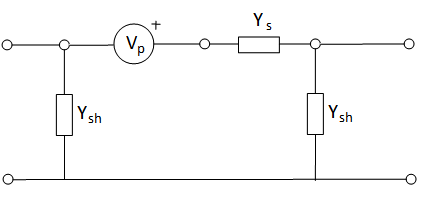
\includegraphics[scale=0.6]{./Figures/pi_section.png}
\end{center}
\end{figure}

Multiple subsections are pieced together in series to obtain the final pipeline circuit model. Shunt connections to earth can also be added to subsections to represent pipeline earthing impedances. Consider the two section pipeline model in Figure \ref{fig:two_section} that is earthed at one end by a resistance $R_g$ (shown in the figure as an admittance $Y_g$).

\begin{figure}
\begin{center}
\caption{Two section pipeline circuit earthed at one end}
\label{fig:two_section}
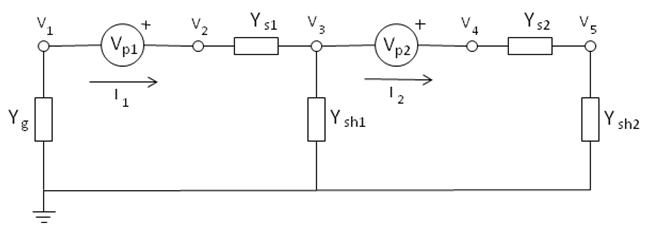
\includegraphics[width=\linewidth]{./Figures/two_section_pipe.png}
\end{center}
\end{figure}

Node voltage equations can be developed as follows:
\\ \\
\hphantom{whe}At Node 1: $V_1 Y_g + I_1 = 0$ \\ \\
\hphantom{whe}At Node 2: $(V_2 - V_3)Y_{s1} - I_1 = 0$ \\ \\
\hphantom{whe}At Node 3: $-(V_2 - V_3)Y_{s1} + V_3 Y_{sh1} + I_2 = 0$ \\ \\
\hphantom{whe}At Node 4: $(V_4 - V_5)Y_{s2} - I_2 = 0$ \\ \\
\hphantom{whe}At Node 5: $-(V_4 - V_5)Y_{s2} + V_5 Y_{sh2} + I_2 = 0$ \\

The induced pipeline voltages in terms of the node voltages are:
\\ \\
\hphantom{whe}$V_{p1} = V_2 - V_1 $ \\ \\
\hphantom{whe}$V_{p2} = V_4 - V_3 $ \\

This linear system of equations can be represented in matrix form as follows:

\begin{equation}
\begin{bmatrix}
Y_g & 0 & 0 & 0 & 0 & 1 & 0 \\
0 & Y_{s1} & -Y_{s1} & 0 & 0 & -1 & 0 \\
0 & -Y_{s1} & Y_{s1} + Y_{sh1} & 0 & 0 & 0 & 1 \\
0 & 0 & 0 & Y_{s2} & -Y_{s2} & 0 & -1 \\
0 & 0 & 0 & -Y_{s2} & Y_{s2} + Y_{sh2} & 0 & 0 \\
-1 & 1 & 0 & 0 & 0 & 0 & 0 \\
0 & 0 & -1 & 1 & 0 & 0 & 0
\end{bmatrix}
\begin{bmatrix}
V_{1} \\ V_{2} \\ V_{3} \\ V_{4} \\ V_{5} \\ I_{1} \\ I_{2}
\end{bmatrix}
=
\begin{bmatrix}
0 \\ 0 \\ 0 \\ 0 \\ 0 \\ V_{p1} \\ V_{p2}
\end{bmatrix}
\end{equation}

The shunt potentials ($V_1$, $V_2$, $V_3$ and $V_4$) and series currents ($I_1$ and $I_2$) can then be solved by normal matrix techniques.

The preceding analysis for a two section pipeline can be extended to an arbitrary number of pipeline sections (for example, the n-section model in Figure \ref{fig:pipeline_model}).

\begin{figure}[!htp]
\begin{center}
\caption{Pipeline circuit model with n sections}
\label{fig:pipeline_model}
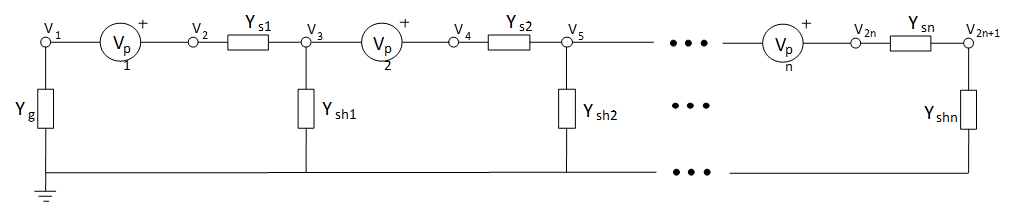
\includegraphics[width=\linewidth]{./Figures/pipeline_model.png}
\end{center}
\end{figure}

\newpage
\section{Using the Program}
\subsection{Right of Way Tab}
The Right of Way tab describes the plan layout of the overhead line in relation to the pipeline. It also allows the user to specify the points on the pipeline that are intentionally earthed, the soil resistivity of each pipeline section and the phase rotation of the overhead line conductors (i.e. to allow for transpositions). 

\begin{figure}[!htp]
\begin{center}
\caption{Right of way tab}
\label{fig:right_of_way}
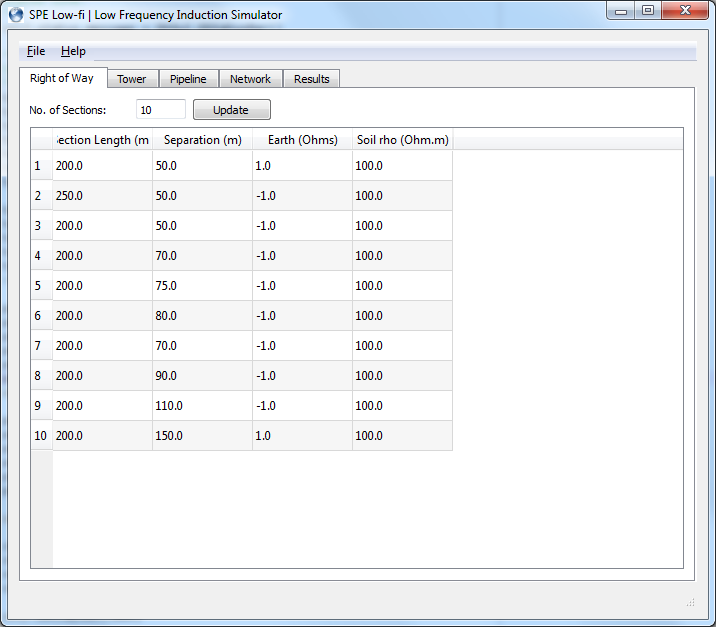
\includegraphics[width=0.9\linewidth]{./Figures/right_of_way.png}
\end{center}
\end{figure}

\begin{itemize}
\item The horizontal separation distance and the earthing impedance is nominated at the start of the section
\item For each section, the geometric average separation distance is calculated based on the separation distances for the current section and the next section
\item For the final section (where there is no next section) or where the next section is non-parallel, the separation distance is assumed to be constant for the entire sectional length
\item A separation distance $<$0 indicates that the pipeline is not parallel to the overhead line
\item An earthing impedance $<$0 indicates that the start of the pipeline section is not intentionally earthed. Earthing impedances can be real or complex values. For complex impedances, use the 'j' operator, e.g. $0.5 + 0.4j \Omega$
\item The phasing field indicates the phase rotation of the overhead line conductors to allow the modelling of line transpositions. Each field is a dropdown box indicating no phase rotation, a 120 degree phase rotation or a 240 degree phase rotation. 
\end{itemize}

\subsection{Tower Tab}
The Tower tab describes the geometry of the overhead line tower with respect to a buried pipeline. Distances are either relative to the closest phase conductor to the pipeline (i.e. phase 'a') or the pipeline. Note that the horizontal separation distance between phase 'a' and the pipeline is specified in the Right of Way tab for each sectional length.

\begin{figure}[!htp]
\begin{center}
\caption{Tower geometry tab}
\label{fig:tower}
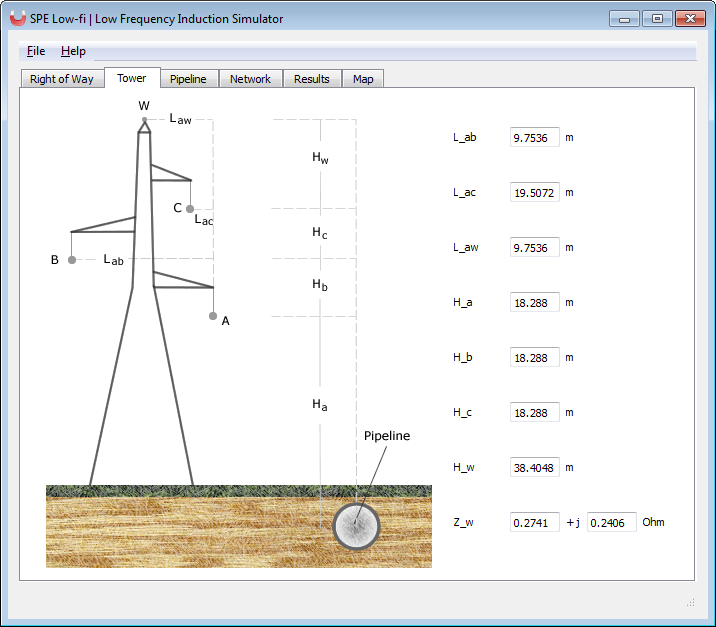
\includegraphics[width=0.9\linewidth]{./Figures/tower_geometry.png}
\end{center}
\end{figure}

\begin{itemize}
\item $L_{ab}$ is the horizontal distance between phase conductors 'a' and 'b' (m)
\item $L_{ac}$ is the horizontal distance between phase conductors 'a' and 'c' (m)
\item $L_{aw}$ is the horizontal distance between phase conductor 'a' and the earth wire (m) - Note 1
\item $H_a$ is the height of phase conductor 'a' from the pipeline (m)
\item $H_b$ is the height of phase conductor 'b' from the pipeline (m)
\item $H_c$ is the height of phase conductor 'c' from the pipeline (m)
\item $H_w$ is the height of the earth wire from the pipeline (m) - Note 1
\item $Z_w$ is the series self impedance of the earth wire ($\Omega$/km)
\end{itemize}

Note 1: to model overhead lines without earth wires, set either of the earth wire parameters $L_{aw}$ or $H_w$ to a negative number.

\subsection{Pipeline Tab}
The Pipeline Tab allows the user to input the pipeline and coating material characteristics, which will be used to compute the series impedance and shunt admittance of the pipeline (refer to section \ref{sec:pipeline_impedance} for more details).

\begin{figure}[!htp]
\begin{center}
\caption{Pipeline details tab}
\label{fig:pipeline}
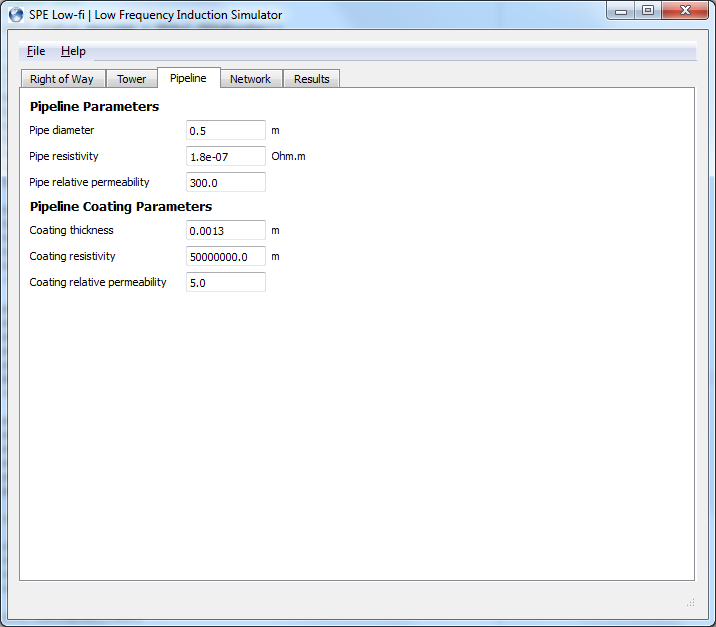
\includegraphics[width=0.9\linewidth]{./Figures/pipeline.png}
\end{center}
\end{figure}

\begin{itemize}
\item Pipe diameter is the cross-sectional diameter of the pipeline (m)
\item Pipe resistivity is the resistivity of the pipeline metal / material ($\Omega$.m)
\item Pipe relative permeability (pu)
\item Coating thickness is the thickness of the coating layer (m)
\item Coating resistivity is the resistivity of the coating material ($\Omega$.m)
\item Coating relative permeability (pu)
\end{itemize}

\subsection{Network Tab}
The Network tab describes the relevant power system characteristics of the overhead line under both normal load and fault conditions.

\begin{figure}[!htp]
\begin{center}
\caption{Network data tab}
\label{fig:network}
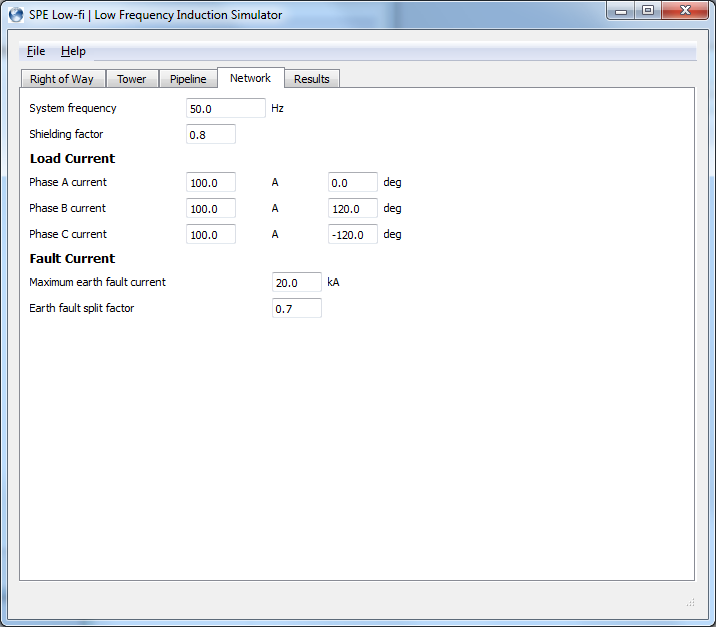
\includegraphics[width=0.9\linewidth]{./Figures/network.png}
\end{center}
\end{figure}

\begin{itemize}
\item System frequency is the nominal power frequency of the current flowing through the overhead line (Hz)
\item Shielding factor is a scaling factor used to capture shielding effects due to multiple pipelines and overhead earth wires (pu)
\item Load current describes the normal operating load currents per phase flowing through the overhead line (A)
\item Maximum earth fault current is the maximum short circuit current magnitude that is expected from an earth fault where the fault current flows along the entire joint right of way (kA)
\item Earth fault split factor is the proportion of current that returns through the earth (pu). The rest of the fault current is assumed to return through the overhead earth wires.
\end{itemize}

\subsection{Results Tab}
The Results tab displays the simulation results (in terms of pipeline-to-earth touch voltages at each section) for load and fault LFI cases. When the "Calculate" button is pressed, a table of the LFI voltages are displayed (see Figure \ref{fig:results_after_calc}) and a plot of the LFI voltages is also automatically generated (see Figure \ref{fig:results_plot}). 

\begin{figure}[!htp]
\begin{center}
\caption{Results tab before calculation}
\label{fig:results_before_calc}
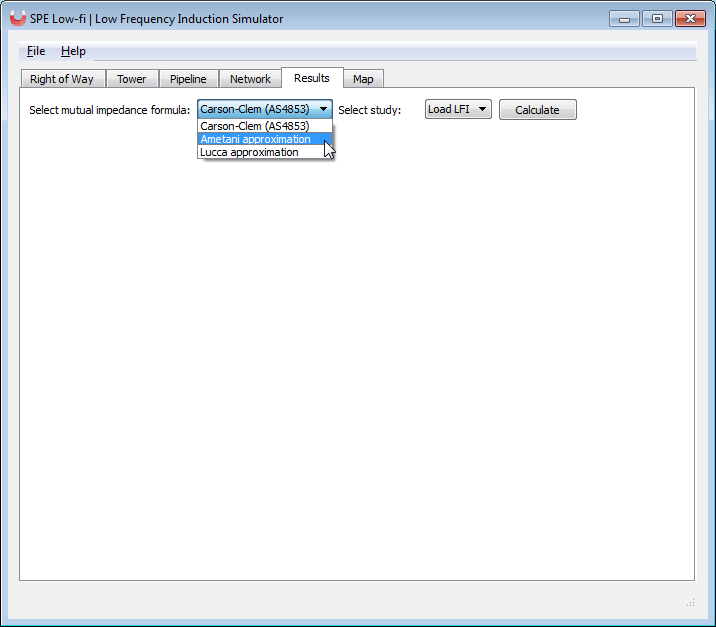
\includegraphics[width=0.9\linewidth]{./Figures/results_1.png}
\end{center}
\end{figure}

\begin{figure}[!htpb]
\begin{center}
\caption{Results tab after calculation}
\label{fig:results_after_calc}
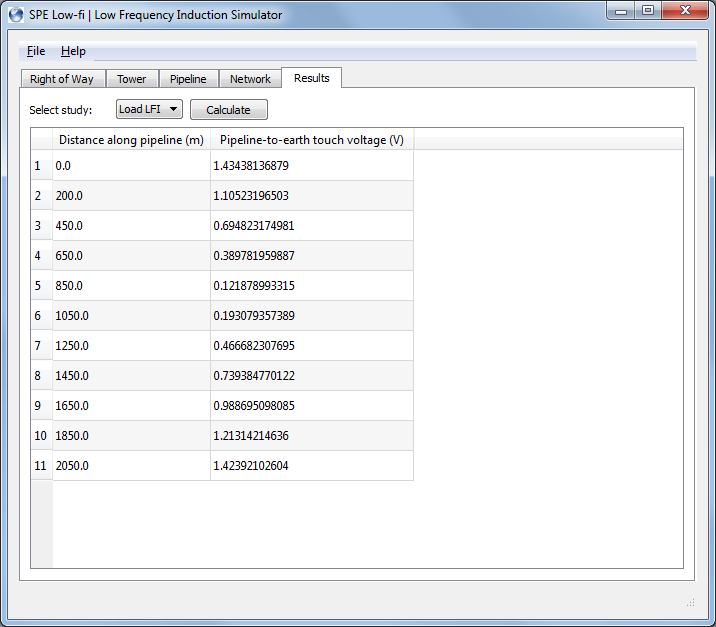
\includegraphics[width=0.7\linewidth]{./Figures/load_lfi_results.png}
\end{center}
\end{figure}

\begin{figure}[!htpb]
\begin{center}
\caption{Load LFI simulation plot}
\label{fig:results_plot}
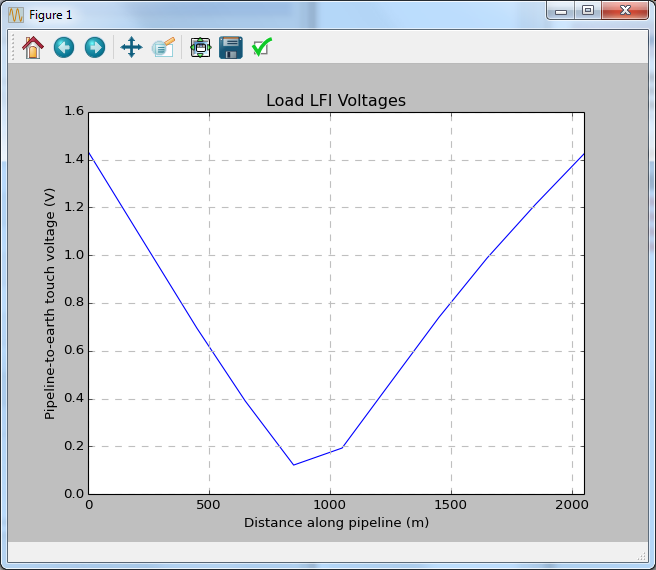
\includegraphics[width=0.7\linewidth]{./Figures/load_lfi_plot.png}
\end{center}
\end{figure}

\newpage
\subsection{Saving and Opening Data Files}
You can save and open \textbf{Low-fi} data files from the File menu. \textbf{Low-fi} data files capture all of the input information entered in the Right of Way, Tower, Pipeline and Network tabs. 

\begin{figure}[!htpb]
\begin{center}
\caption{Saving and opening \textbf{Low-fi} data files}
\label{fig:saveload}
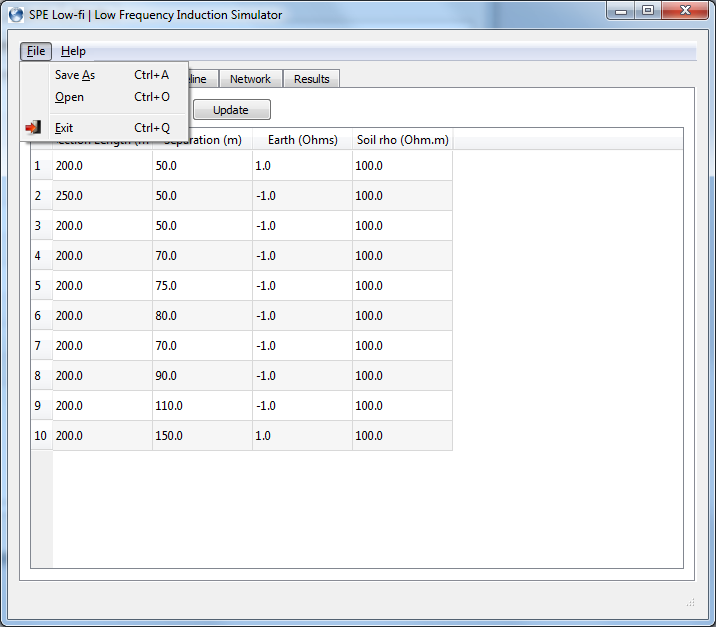
\includegraphics[width=0.9\linewidth]{./Figures/RoW_with_file_menu.png}
\end{center}
\end{figure}

\newpage
% Bibliography
\bibliographystyle{plain}
\bibliography{bib_refs}

\end{document}
